\section{Study 2: How Does RePlay Compare to Current Methods for Video Assistance?}
\label{sec:replay_study}

A between-subjects study ($n\!=\!24$) investigated how contextual assistance for multi-app activities might affect behavior compared to standard web video search. It found that contextual assistance can reduce time spent searching and navigating videos.

\subsection{Study Procedure}

\begin{figure*}[b!]
\centering
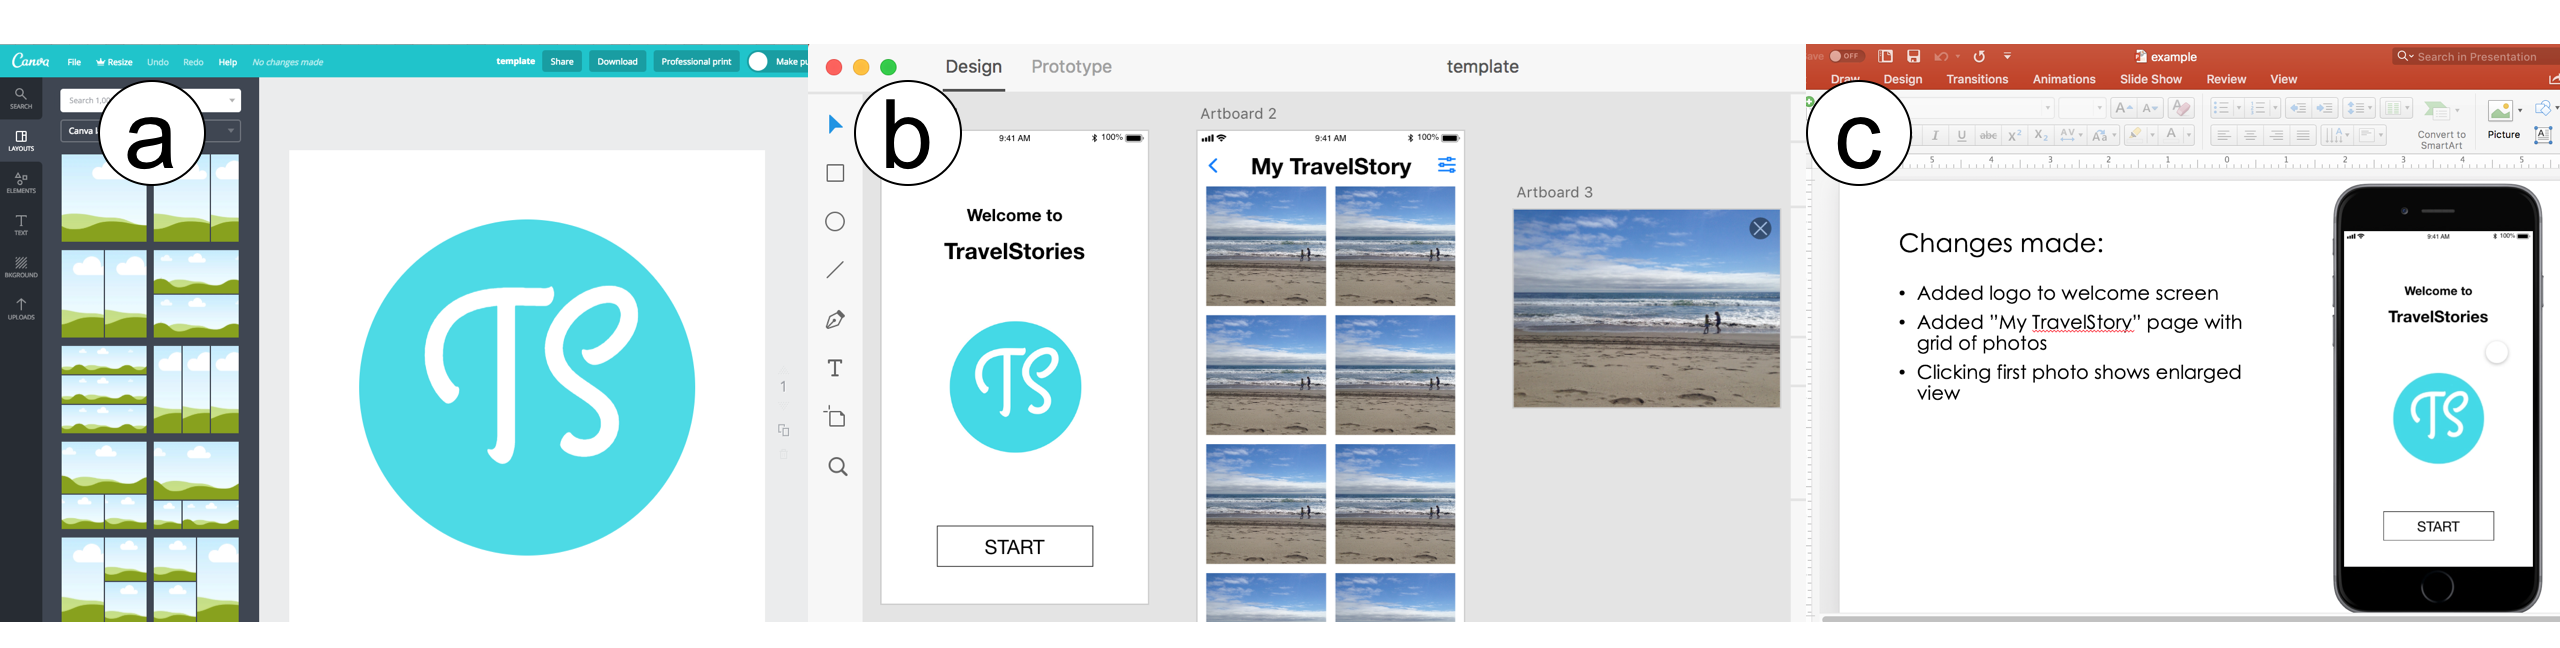
\includegraphics[width=\textwidth]{replay/figures/study2_task.png}
  \caption{Study 2 asked participants to make changes to an initial logo in Canva (a), update a prototype in Adobe \textsc{xd} (b), and make a presentation showing their changes in PowerPoint (c).}~\label{fig:replay-study2-task}
%   \Description[Screenshots of the three template files participants were given.]{Screenshots of the three template files participants were given. The first is a blue circle with ``TS'' in the middle, shown in the Canva interface. The second is a wireframe design in Adobe XD with three phone screens, one that says ``Welcome to TravelStories'' with a Start button, one that says ``My TravelStory'' with a grid of photos below it, and one showing a photo at full size. The third is slide in PowerPoint with a screenshot of the wireframe on the right, and some text on the right that lists changes made to the design.}

\end{figure*}

Participants were asked to imagine that they were designers working for a client developing a travel journal mobile app. To replicate a multi-app activity, the study task spanned three applications: Canva (\href{https://canva.com}{\nolinkurl{canva.com}}), Adobe \textsc{xd}, and Microsoft PowerPoint. Participants were asked to improve and change an initial design for their client (\autoref{fig:replay-study2-task}). The task had both creative and technical requirements. Creative requirements included making the logo more travel-themed, adding visual appeal to the prototype welcome screen, and making a PowerPoint presentation to show to the client. Technical requirements included adding additional photos to a grid, rounding their corners, and recording a video walkthrough. If participants needed help, they were instructed to search for tutorial videos using either RePlay or YouTube in a web browser. RePlay participants were introduced to its features prior to the task. To ensure that all participants had access to the same resources, they were asked not to use other search engines or resources. Participants had 45 minutes to complete the task, and answered questions about their experience and help-seeking at the end. Participants were compensated with a \$15 gift card.

\subsubsection{Participants}
Twenty four participants (14 female) were recruited through online and paper advertisements on a university campus. Prior to the study, participants filled out a survey about their design experience. Participants were randomly assigned to either the RePlay ($n\!=\!12$) or Web ($n\!=\!12$) condition and counterbalanced based on experience. ``Novice'' was defined as completing at most two courses in design and reporting experience with at most two design applications. ``Experienced'' was defined as completing more than two courses in design or reporting experience with more than two design applications. Six of the 24 participants were ``experienced''. 

Participants rated their pre-study familiarity with each of the three study applications on a 5-point Likert Scale. Participants were generally familiar with Powerpoint ($mean\!=\!4.2$), and unfamiliar with Canva ($mean\!=\!1.5$) and Adobe \textsc{xd} ($mean\!=\!1.2$).
 
\subsubsection{Measures}
We were primarily interested in participants' search behavior. We measured the number of queries, their length, and time spent in the search interface. Qualitative measures included how participants determined which videos to watch and their navigation strategies (observed through screen recordings). We also gathered participant feedback in the RePlay condition on its features.

\subsection{Results}
RePlay participants averaged 3.3 queries each (33 total); Web participants averaged 3 queries each (24 total) ($x^2\!=\!1.42$, $df\!=\!1$, $p\!=\!.23$). Web participants typed longer queries ($mean\!=\!4.33$ words, $SD\!=\!1.41$) than RePlay participants ($mean\!=\!2.53$ words, $SD\!=\!0.59$)($t\!=\!2.52$, $df\!=\!15.98$, $p\!<\!.01$), because Web participants often manually added the application name, whereas RePlay auto-included it. 72\% of search queries were for Adobe \textsc{xd} and 28\% were for Canva; none were for PowerPoint since participants were more familiar with it. Four Web and two RePlay participants did not search for any assistance; we cover this in the Discussion.

Participants varied considerably in the amount of time and effort they spent. This is a challenge with a task that has both creative and technical components; people prioritize these components differently. Many participants spent a long time perfecting their design and had to be cut off after 45 minutes; others did the minimum required and finished in as few as 23 minutes. Because the task was open-ended, we did not compare completion times across participants. Our analysis focuses on search behavior. 

\begin{figure}[b!]
\centering
%\vspace{-0.25in}
  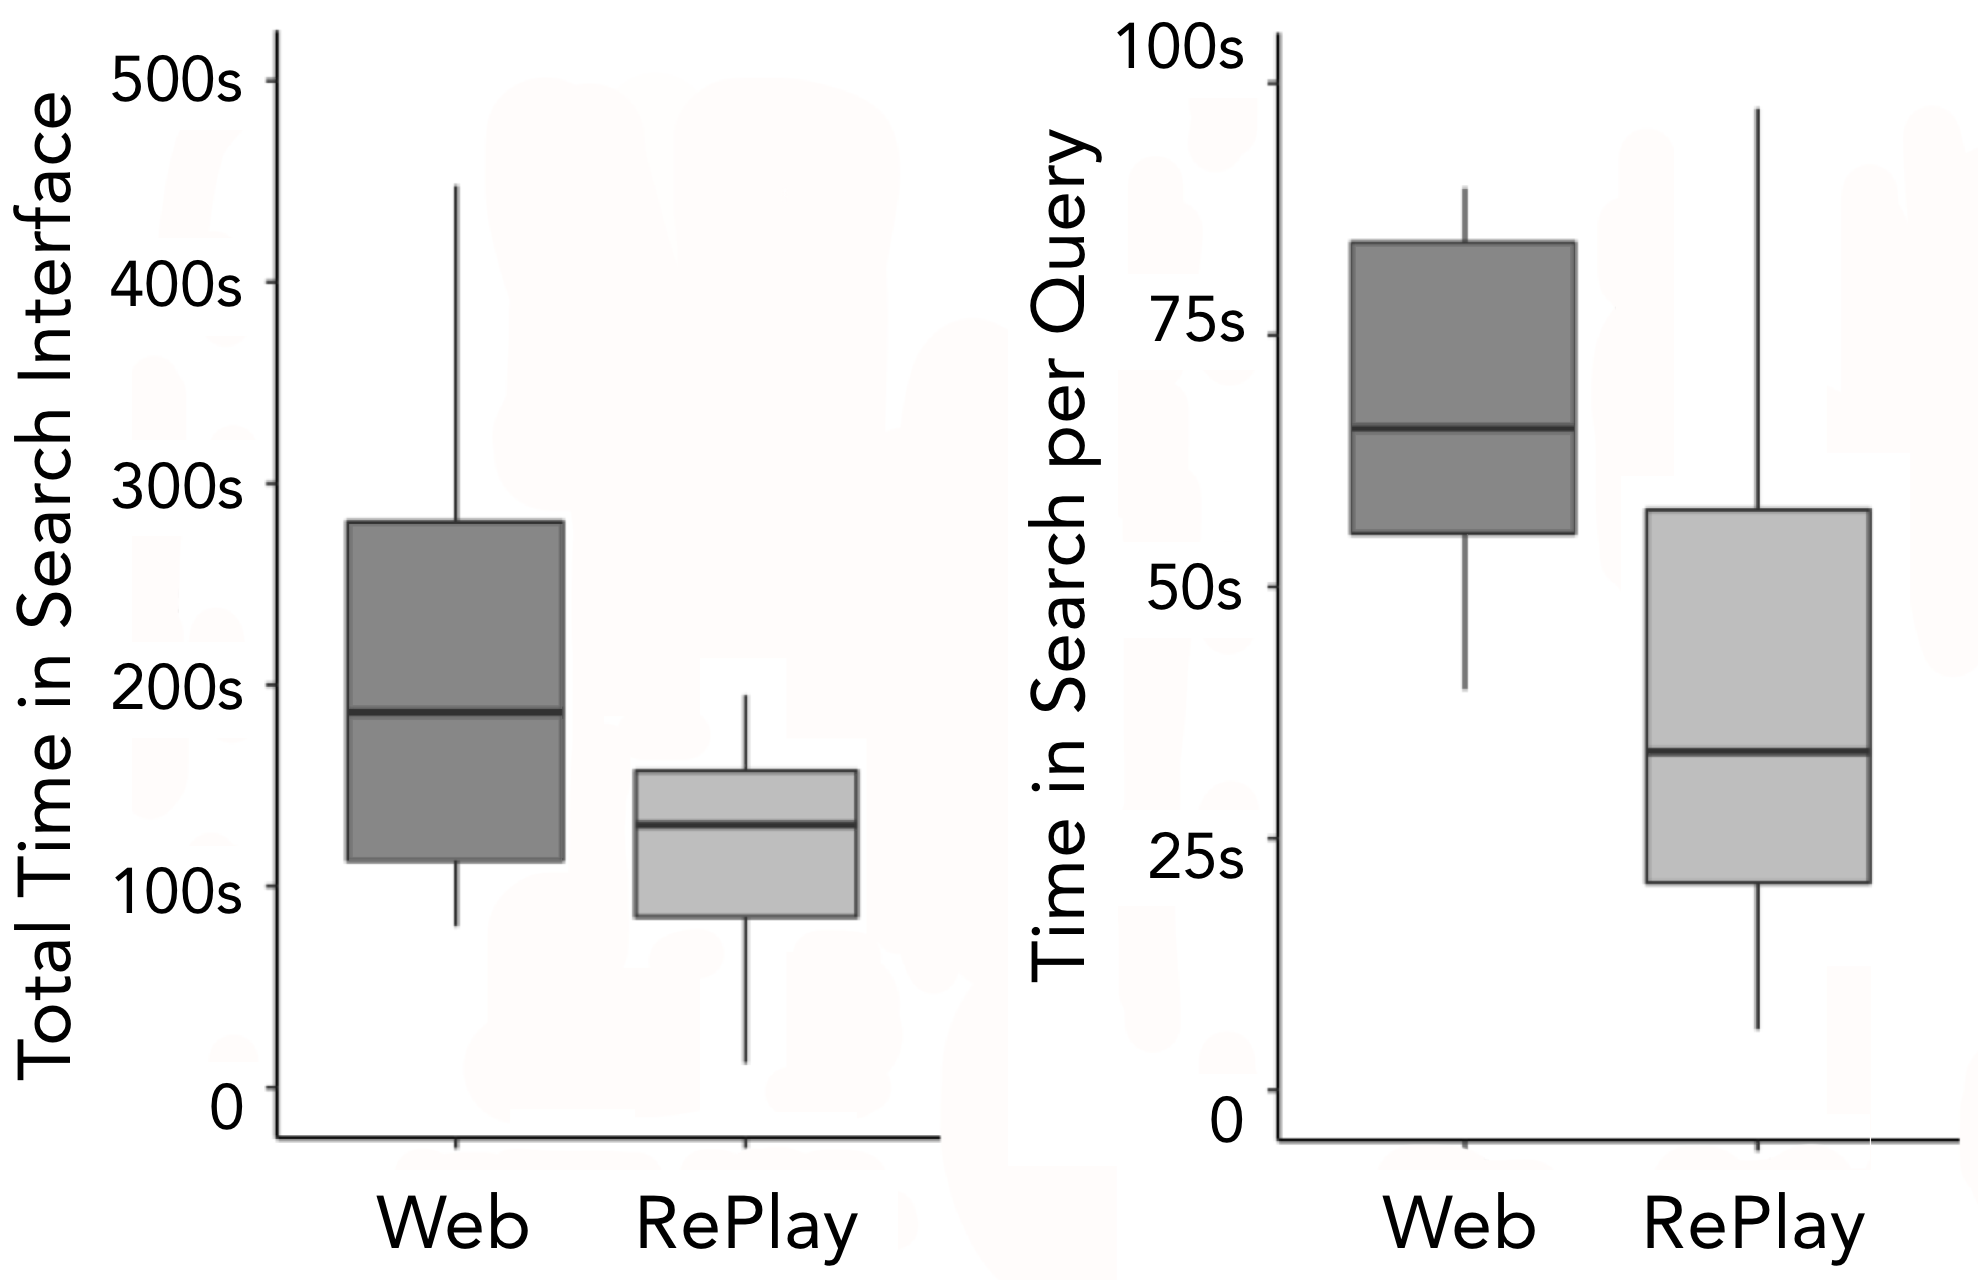
\includegraphics[width=.8\textwidth]{replay/figures/study2_graphs.png}
  \caption{RePlay participants spent marginally less time overall in the search interface than Web participants ($p\!=\!.07$, left) and significantly less time \textit{per query} ($p\!=\!.02$, right).}~\label{fig:replay-study2-graphs}
%   \Description[Two graphs showing the difference between RePlay and Web participants in time spent in the search interface.]{Two box plots showing the difference between RePlay and Web participants in time spent in the search interface. On the left, RePlay's box is slightly lower than Web's for total time in search (seconds). On the right, RePlay's box is significantly lower than Web's for time in search by query per person (seconds).}
\end{figure}

% Keep this somewhere? As a result, traditional completion time or completion rate are not suitable metrics. 

\subsubsection{Contextual assistance lessens time away from task}
Web participants spent nearly twice as long in the search interface ($mean\!=\!214.5$ seconds, $SD\!=\!127.1$) as RePlay ones ($mean\!=\!116.2$ seconds, $SD\!=\!58.9$). Due to the high variance and small sample size, the difference was marginally significant ($t\!=\!2.02$, $df\!=\!9.4$, $p\!=\!.07$) (\autoref{fig:replay-study2-graphs} left). When the time each participant spent in search is averaged by the number of queries they made, the difference is significant: RePlay participants spent about 40\% less time in search per query ($mean\!=\!42.83$ seconds, $SD\!=\!29.5$) than Web participants ($mean\!=\!72.62$ seconds, $SD\!=\!22.4$)($t\!=\!2.52$, $df\!=\!15.28$, $p\!=\!.02$) (\autoref{fig:replay-study2-graphs} right). Though RePlay pre-cached many video captions beforehand, we could not predict all queries users would make. Thus, some query responses in RePlay took up to two minutes. Because this latency could be reduced, we subtracted loading times in both conditions from the total time in search.

Easier navigation both within and between video results may explain why RePlay participants spent less time in the search interface per query. Web participants used various strategies for navigating within videos, including keyboard shortcuts to fast-forward and rewind, increasing video speed, and hovering over the timeline. Navigating between different video results in YouTube required selecting a video, watching or skipping through it to determine whether it was relevant, and if not, going back to the results page and selecting another. RePlay's timeline markers replaced many of these strategies, increasing efficiency: participants could first examine the timeline markers before deciding if and at what point to watch a video result. Eight RePlay participants hovered over timeline markers to read the caption previews, often hovering over multiple points before deciding where to watch. RePlay's panel interface also enabled participants to simultaeously play one video and examine others. We observed three participants do this, likely to decide whether another video was better without giving up on their first choice. One such participant said they wished for better visual cues of video relevance to help decide which to watch. Other participants browsed videos one at a time, perhaps to focus on the playing video.

% \begin{figure}[b!]
% \vspace{-0.25in}
% \centering
%   \includegraphics[width=0.9\textwidth]{replay/figures/study2_avgsearch.png}
%   \caption{Web participants spent significantly longer in the search interface \textit{per search query} than RePlay participants ($p=.02$). }~\label{fig:replay-study2-avgsearch}
% \end{figure}

\subsubsection{Search queries were action-oriented, not tool-oriented}
As in Study 1, participants removed tool names from queries. No participants in either condition used tool names. Instead, participants wrote action-oriented queries: the most common were ``crop photos'', ``round corners'', and ``record video.'' Despite RePlay adding the current tool name to the search field, in all instances but one, participants deleted the tool name from their query.

\begin{table}[t]
\centering
\caption{Average helpfulness ratings for RePlay's contextual features ($n\!=\!12$). Most participants found the timeline markers most helpful for determining which videos to watch.}~\label{table:replay_study2_features}
\begin{tabular}{lllll}
\textit{RePlay Feature} & Title                   & Thumbnail               & Caption                 & Timeline                \\ 
\textit{Helpfulness}    & \multicolumn{1}{c}{2.8} & \multicolumn{1}{c}{3.1} & \multicolumn{1}{c}{2.5} & \multicolumn{1}{c}{4.2}
\end{tabular}
\end{table}

\subsubsection{Intra-video context is most helpful}
In interviews, participants rated timeline markers as the most helpful (4.2/5) (\autoref{table:replay_study2_features}). RePlay participants hovered over timeline markers a total of 69 times and clicked on markers 22 times. One participant mentioned that timeline markers provide a \textit{``scaffold of what to look for and where to start watching.''} Participants rated caption excerpt and video title as less helpful. A few participants mentioned ignoring titles and excerpts in favor of timeline markers and video thumbnails. Twice in each condition, participants selected the first video result even though the title mentioned the wrong application (Photoshop or Illustrator). This suggests that the video region is a strong magnet for people's attention.


%Tasks that require a context switch are perceived to take longer than tasks that don't. 
%Intra-person effect size for search interfaces is smaller than inter-person differences. To see the impact of search interfaces, need large n.
% One motivation for having the app do searching for you is that people aren't good at it. 

% Another participant found the timeline markers helped them \textit{extrapolate form the video where I should search for the content that I'm looking for. And it that one doesn't have it, I can just skip through and see other [points].''} general, participants found this feature helpful (4.11 rating on 5-point Likert scale). 